\section{Graph-based Machine Learning}
\label{sec:graph-based-machine-learning}

We formulate our system in a Message Passing Neural Network (MPNN)
framework~\cite{Gilmer2017,Li2015a} and implement a single unified
model for all our experiments. Our design mimics the \emph{transfer
  functions} and \emph{meet operators} of classical iterative dataflow
analysis~\cite{Kam1977,Cooper2003}, replacing the rule-based
implementations with deep learning analogues (message and update
functions). Those can be specialized through training to solve a
diverse set of problems without human intervention or algorithm
design.


\subsection{Overview}

We learn over \textsc{ProGraML} representations of compiler IRs by
mapping graph vertices to an initial state vector using an
embedding. The vertex states are updated iteratively in a sequence of
message passing steps, where at each step a new vertex state is
computed as a function of its previous state and the state of its
neighboring vertices. Separate functions are learned to update vertex
neighbors based on their relation type, be it control, data or call,
and reverse edges enable backwards propagation of information. After
repeating this process of updating vertex states for a fixed number of
iterations a readout function is used to aggregate the vertex
representations to a single graph-level vector or set of vertex-level
vectors.


\subsection{Model Design}

The \textsc{ProGraML} model takes as input a directed graph with
additional information as presented in
Section~\ref{sec:graph-representation} and consists of three logical
phases: input encoding, message propagation, and result readout.

\paragraph{(I) Input Encoding} Starting from the augmented graph
representation $G = (V, E)$ introduced in Section
\ref{sec:graph-representation}, we capture the semantics of the
program graph vertices by mapping every instruction, constant, and
variable vertex $v \in V$ to a vector representation
$h_v^0 \in \mathbb{R}^{d}$ by lookup in a fixed size embedding table
$C_ \text{IR} \in \mathbb{R}^{n \times d}$. The mapping from vertex to
embedding vector $f: v \hookrightarrow h_v^0 \in C_\text{IR}$ must be
defined for each IR, though the embeddings themselves can be learned
during training.

For LLVM-IR we extend the inst2vec~\cite{Ben-nun2018} vocabulary,
which represents 8,566 statements derived from a large corpus of
LLVM-IR using 200-dimensional embeddings. Since the space of
statements is unbounded, inst2vec uses a normalization process to
inline type definitions and strip identifiers and immediate values,
depicted in Figure~\ref{fig:embedding}. An inst2vec representation
combines an instruction and its operands into a single token, so we
augment the vocabulary with \textsc{Id} and \textsc{Val} tokens to
represent variable and constant value vertices, respectively.

In expressing a statement as a combination of an instruction and its
operands, our data-driven approach trades a certain amount of semantic
resolution against good coverage of the vocabulary by the available
datasets. The long tail of the distribution of statements jointly maps
onto a special \textsc{Unknown} token vector in the vocabulary. In
future work will simplify the LLVM-IR statement encoding by
constructing separate vocabularies for instructions and operand types,
increasing the expressiveness of the encoding by allowing a larger
combination of instruction and operands to be represented.  Input
\emph{vertex-selectors}, encoded as binary one-hot vectors, are used
to mark the starting point for certain analyses and are concatenated
to the vertex
embeddings.
Other global input features are used as auxiliary input features at
readout time in step (III), where required.

\begin{figure}
  \centering
  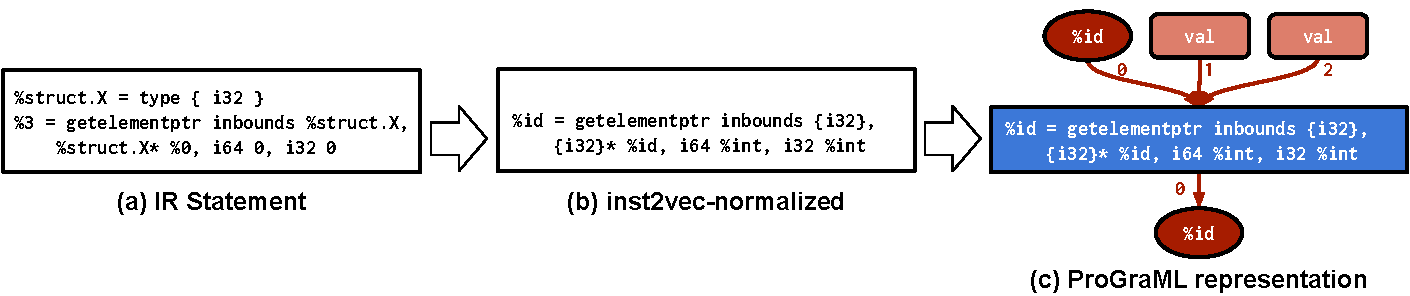
\includegraphics[width=\linewidth]{images/embedding}%
  \caption{%
    Normalizing an LLVM-IR statement (a) by inlining type definitions
    and stripping identifiers using inst2vec~\cite{Ben-nun2018} (b). A
    normalized statement is used as the key for an embedding table
    lookups to produce the initial vector representation of a
    vertex. (c) shows the statement as contextualized in a
    \textsc{ProGraML} graph, where the operand variables and constants
    are data elements, differentiated by their position. Vertex labels
    represent embedding table keys. In this example, the statement is
    represented using five vertices and encoded with three unique
    embeddings.%
  }%
  \label{fig:embedding}%
\end{figure}

\paragraph{(II) Message Propagation} Each iteration step is divided
into a message propagation step followed by a vertex state
update. During message propagation, each vertex in the graph collects
learned messages $m_v^{t} \in \mathbb{R}^d$ from its undirected
neighbors:

\begin{equation}
  m^t_{v} = \sum_{w \in \mathcal{N}(v)} A_{\mathrm{type}(e_{wv})}\,  (h_w^{t-1} \odot \textsc{pos}(e_{wv}))\,
\end{equation}

where $\odot$ denotes the Hadamard product and $e_{wv} \in E$ is the
typed edge between vertex $w$ and $v$. In order to allow for
reverse-propagation of messages, which is necessary for backward
compiler analyses, we add backward edges for each edge in the
graph. For backward edges we introduce separate parameters following
Li et al.~\cite{Li2015a} to enable the network to distinguish between
an edge and its backward sibling. During message propagation we scale
the source states $h_v^{t-1}$ with
\textsc{pos}$(\cdot) \in \mathbb{R}^d$, which is a constant sinusoidal
position embedding~\cite{Vaswani2017,Gehring2017} that encodes the
argument order of incoming (and outgoing) edges. This information is
necessary for the network to distinguish non-commutative operations
such as division.

The collected messages are subsequently used to update the vertex
states $h_{v} \in \mathbb{R}^d$ in parallel according to an update
function. In all our experiments, we employ a Gated Recurrent Unit
(GRU) \cite{Cho2014} as our update function:

\begin{equation}
h_v^t = \textsc{Gru}(h_v^{t-1}, m_v^t)
\end{equation}

Step (II) is iterated $T$ times to extract vertex representations that
are contextualized with respect to the given graph structure.

\paragraph{(III) Result Readout} We support whole program
classification, per-statement classification, or per-identifier
classification by employing different \emph{readout heads} on top of
the iterated feature extraction: for graph-level classification we
define a set function $R_G(\{h_v^T, h_v^0\}_{v \in V})$ that maps to
class-scores, while for vertex-level inference, we separately map the
extracted node features $h_v^T$ to probabilities $R_v(h_v^T, h_v^0)$
in parallel:
\begin{align}
  R_{v}(h_v^T, h_v^0) &= \sigma\left(i(h_v^T, h_v^0)\right) \cdot j(h_v^T) \\
  R_{G}(\{h_v^T, h_v^0\}_{v \in V}) &= \sum\limits_{v \in V}\,\,R_{v}(h_v^T, h_v^0)
\end{align}
where $i(\cdot)$ and $j(\cdot)$ are feed forward Neural Networks and
$\sigma(\cdot)$ is the sigmoid activation function.  In the case where
auxiliary graph-level features are available, those are concatenated
to the readout values and fed through another feed forward Neural
Network that employs Batch Normalization~\cite{Ioffe2015a} to allow
for vastly different feature scales.
